\newpage
\section{Introduction}

\subsection{Background}
“Expert Finding Systems (EFS) [or \ac{EFS}], also called \ac{ELS} enable users to discover subject matter experts in order to hire or acquire their 
knowledge.” (\cite[page vii]{maybury_expert_2006}) It is an important asset especially for big corporations, as it can boost efficiency and lower the barrier of 
entry for new employees. First appearances of \ac{EFS} can be traced back to the papers “Enterprise expert and knowledge discovery” (\cite{mattox_enterprise_1999}) and 
“Facilitating the Online Search of Experts at NASA Using Expert Seeker People-Finder” (\cite{becerra-fernandez_facilitating_nodate}) . Further research has been 
conducted by Mark T. Maybury in his Paper “Expert Finding Systems” (\cite{maybury_expert_2006}). The National Forum on Expert Finding Systems states Research 
Gate, LinkedIn or Harvard Catalyst Profiles as current examples of \ac{EFS}. (\cite{noauthor_national_nodate})
\\ \\
While examples like Research Gate or LinkedIn are more 
general approaches to \ac{EFS}, corporations face the challenge of implementing \ac{EFS} that fit their specific needs and organizational structures.
Four of the most commonly used organizational structures are the functional structure, which focuses of a clear chain of command and separates the organization 
into different departments based of their expertise (\cite{noauthor_what_nodate-1}) , a product- or market-based structure where different departments are based on 
different products or markets instead of expertise, the geographical structure which divides teams based on their location and a process based structure which 
groups the employees into teams based on the business processes they are engaging in. (\cite{organ_7_2023})   
An alternative approach is the matrix structure. The matrix structure is on the rise with 84\% of employees being “matrixed” in some way according to a study of 
cross-functional teams conducted by Gallup. (\cite[page 65]{inc_state_nodate}) The Matrix organization stands out by having multiple lines of reporting, meaning 
that employees have two or more bosses effectively. (\cite{noauthor_what_nodate})(\cite{organ_7_2023}) This makes the Matrix organization a great match for agile working and cross functional teams. The main challenge that needs to be addressed regarding an \ac{EFS} in a Matrix organization are dynamic and constantly changing tasks and fields of expertise, as people are incentivized to grow in those environments.
Therefore, an \ac{EFS} has to be able to handle those constant changes in ability, especially because it nearly impossible for the employees to keep track of all their 
colleagues’ skills over time.
\\ \\
Technologische Grundlagen (AI, …)\\
The efficiency of \ac{EFS} is closely tied to the different technologies that are being used. Therefore the following components and technologies are of interest for the \ac{EFS}:
\begin{itemize}
    \item Reliable data: Data quality is one of the most important factors for the success of an \ac{EFS} as it is the basis for the search algorithm. Some of the
    more popular data sources of commercial tools are Self declared data, Documents and Databases (\cite[page 18]{maybury_expert_2006})
    \item Search algorithm: The search algorithm is the core of the \ac{EFS}. It has to be able to handle the data and provide the user with the most relevant 
    results. Here Keyword search, and Boolean search are the most common methods with the Natural Language Search which utilizes \ac{NLP} being on the third place,
    thogh since the release of the paper by Mark T. Maybury in 2006 (\cite[page 18]{maybury_expert_2006}), \ac{NLP} has gained a lot of popularity especially 
    through the rise of \ac{AI} and Machine Learning with applications in Chatbots, Voice Assistants and Sentiment analysis (\cite{administrator_role_2023}).
\end{itemize}

 Firstly reliable data has to be supplied in order for the \ac{EFS} to work 
properly, making data quality one of the success factors
\\ \\
Geschäftlicher Nutzen?
Forschungslücken


\subsection{Problem Statement}
In an Harvard Business Review article, John Ferraro, the former COO of Ernst \& Young suggests, that in order to keep up with the pace of change, companies have 
to constantly reorganize. (\cite{heidari-robinson_getting_2016}) On the other hand, according to a McKinsey survey, over 80\% fail to deliver the hoped-for value in time, with 10\% even causing real 
damage to the company.(\cite{heidari-robinson_getting_2016}) The article also states that two-thirds of company reorganizations do at lease improve the performance to a degree. (\cite{heidari-robinson_getting_2016}) This suggests that 
there is still some room for improvement regarding the performance. 
This room can be utilized by increasing the efficiency of internal processes with an \ac{EFS} in a few ways. 
This paper evaluates the design and piloting of such an \ac{EFS} at the \ac{T-FOPS} (Figure 1) team at \ac{DTT}. 
\ac{T-FOPS} utilizes a mixture of different organizational structures. On the top-level it is a functionally and partially geographical divided in the sectors 
\ac{T-FOBIZ}, \ac{T-FOC}, \ac{T-FORN} and \ac{T-FORS}, the last two meaning North- and 
South-Germany. The Thesis will focus on \ac{T-FOBIZ} (Figure 2) which is subdivided functionally into the \ac{T-FOBOD}, \ac{T-FOBOS}, 
\ac{T-FOBOT} meaning temporary mobile coverage, and \ac{F-FOBOV} meaning procurement management. 

\begin{figure}[H]
    \centering
    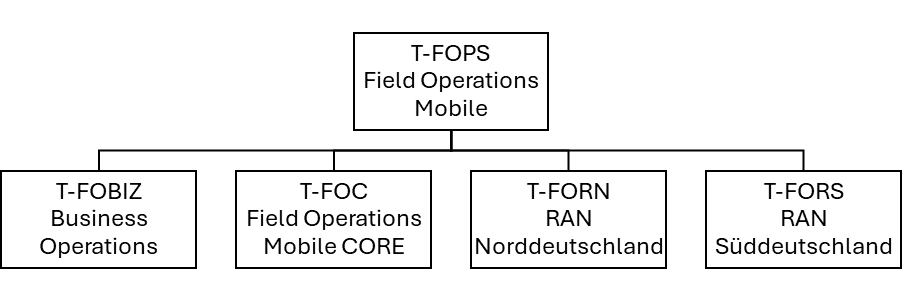
\includegraphics[width=0.7\textwidth]{abbildungen/FopsOrga}
    \caption{Organization Chart \ac{T-FOPS}}
    \label{fig:FopsOrga}
    source: own illustration
\end{figure}
\begin{figure}[H]
    \centering
    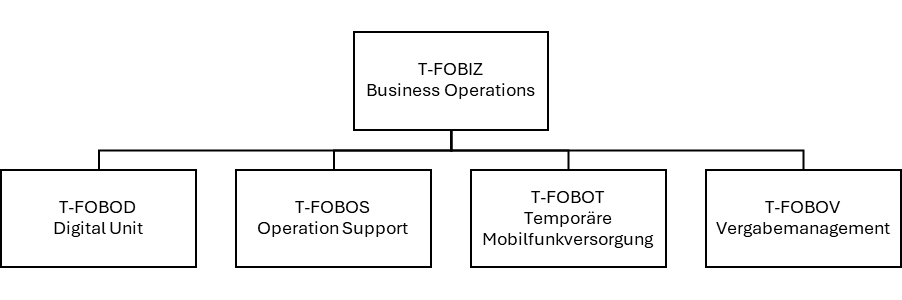
\includegraphics[width=0.7\textwidth]{abbildungen/FobizOrga}
    \caption{Organization Chart \ac{T-FOBIZ}}
    \label{fig:FobizOrga}
    source: own illustration
\end{figure}

\subsection{Structure of the Thesis}

\subsection{Scope and Limitations}

